\documentclass[11pt,letterpaper]{article}

% Load package
\usepackage{lesson}
\usepackage{amsmath}
\usepackage{xcolor}

%--------------------------------------%
% Custom commands include:             %
%%%%%%%%%%%%%%%%%%%%%%%%%%%%%%%%%%%%%%%%
% Include an image:                    %
% \diagram{height}{align}{file}        %
%                                      %
% height: a number representing mm     %
% align: left, center, or right        %
% file: file name without extension    %
%%%%%%%%%%%%%%%%%%%%%%%%%%%%%%%%%%%%%%%%
% Add a numbered question:             %
% \question{text}                      %
% \questiond[lines]{file}{width}{text} %
%                                      %
% lines: # of lines of text to wrap    %
% file: file name without extension    %
% width: a % of textwidth for image    %
%%%%%%%%%%%%%%%%%%%%%%%%%%%%%%%%%%%%%%%%
% Add a lettered option/question part: %
% \option[vspace]{text}                %
%                                      %
% vspace: added space above the option %
%%%%%%%%%%%%%%%%%%%%%%%%%%%%%%%%%%%%%%%%
% Add a blank line in text:            %
% \blankline{width}                    %
%%%%%%%%%%%%%%%%%%%%%%%%%%%%%%%%%%%%%%%%
% Add an arc symbol in math:           %
% \arc{notation}                       %
%--------------------------------------%
%%%%%%%%%%%%%%%%%%%%%%%%%%%%%%%%%%%%%%%%
%--------------------------------------%
% To reset the question counter:       %
% \setcounter{qcounter}{0}             %
%                                      %
% To reset the option counter:         %
% \setcounter{acounter}{0}             %
%--------------------------------------%

% Set title and course name
\settitle{Week 2 Question Set}
\setsubtitle{The Hodgkin-Huxley model \& Eyes}
\setcourse{Summer 2023}

\begin{document}

% Create title and add proper header for first page
\maketitle
\thispagestyle{first}

\section{CNS2.2 - Reversal potential and Nernst equation}
Choose the most correct option for each question:
\begin{enumerate}
    \item Circle the correct choice: At rest, the concentration of K+ is higher (inside/outside) the neuron, and the concentration of Na+ is higher (inside/outside) the neuron.

    \item The video introduces a couple of formulas. Name them and give a brief description.
    \begin{table}[h]
        \centering
        \begin{tabular}{c|c|c}
        \hline
         Formula & \hspace{1 cm} Name \hspace{1 cm} & \hspace{2 cm}\, Brief Description \hspace{2 cm} \,\\
        \hline
        \hline
        $n \propto e^{-E/(kT)}$ &  & \\
        $E = q \cdot u$ & & \\
        $\Delta u = u_{in} - u_{out} = \frac{-kT}{q}\ln\frac{n(u_{in})}{n(u_{out})}$ & & \\
        \hline
        \end{tabular}
    \end{table}

    \item Which of the following statements is correct regarding the Nernst equation and the membrane potential of a neuron? Select all that apply.
    \begin{enumerate}
        \item [a.] The Nernst potential (a.k.a. reverse potential) describes the equilibrium potential for a single ionic species at a time.
        \item [b.] The Nernst potential, also referred to as the reversal potential, is the membrane potential at which the direction of the net flow of a particular ion species across the membrane will reverse.
        \item [c.] The total membrane potential of a neuron is simply a sum of the Nernst potentials for each ion species present.
        \item [d.] The total membrane potential of a neuron at rest is most influenced by the Nernst potential for potassium and sodium, as the membrane is most permeable to those ions.
    \end{enumerate}
\end{enumerate}

\pagebreak

\section{CNS2.3 - Hodgkin-Huxley Model}
\begin{enumerate}
    \item Let's derive the conversation equation of the Hodgkin-Huxley Model:
    \begin{align*}
        I_{stimulus} = C \frac{du}{dt} + g_{Na} \, m^3 h (u - E_{Na}) + g_K \, n^4 (u - E_K) + g_L (u - E_L),
    \end{align*}
    where $g$ are the conductances/permeability of the membrane to the ions, $E$ are the Nernst (equilibrium) potentials, and $m$, $h$, $n$ are gating variables for the sodium and potassium channels.
    \begin{center}
        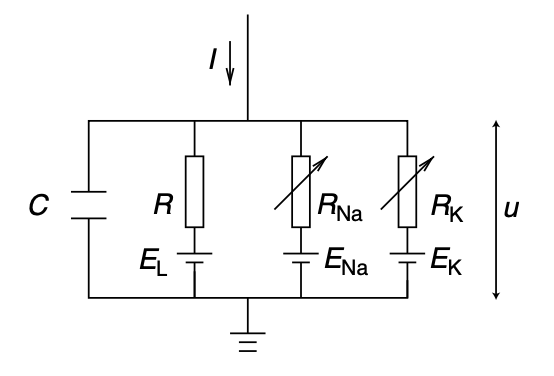
\includegraphics[scale=0.9]{2.3.png}
    \end{center}
    \begin{enumerate}
        \item Start off by using Kirchhoff's Current Law: $I_{stimulus} = I_C + I_{Na} + I_K + I_L$. \emph{Hint}: Feel free to use the following well-known differential equations to simplify the steps:
        \begin{align*}
            I_C = C \frac{du}{dt} \text{  and  } I_n = \frac{u}{R_n}
        \end{align*}
        \vspace{1.2 in}
        \item Then, replace each $1/R$ term with the appropriate conductance and the gating variables.
        \vspace{2 in}
    \end{enumerate}
    \pagebreak

    \item Which of the following statements correctly describe the gating variables in the Hodgkin-Huxley model? Select all that apply.
    \begin{enumerate}
    \item [a.] The gating variables $m$, $h$, and $n$ represent the probabilities that a particular type of voltage-gated ion channel is open.
    \item [b.] The gating variables do not depend on the membrane potential and remain constant over time.
    \item [c.] Each gating variable has an associated rate equation, given by $\frac{dx}{dt} = -\frac{x - x_0(u)}{\tau(u)}$, where $x$ is the gating variable.
    \item [d.]  In this model, $x_0(u)$ is the steady-state value of the gating variable at a given membrane potential, and $\tau(u)$ is the time constant which determines how quickly the gating variable approaches its steady-state value.
    \end{enumerate} 

    \item As the membrane potential $u$ changes, how do the activation and inactivation gating variables typically respond? Please fill in the blanks.
    \begin{enumerate}
    \item An activation gating variable typically (increases/decreases) with an increase in $u$.
    \item An inactivation gating variable typically (increases/decreases) with an increase in $u$.
    \end{enumerate}
\end{enumerate}
\pagebreak

\section{CNS2.4 - Threshold in the Hodgkin Huxley Model}
\begin{enumerate}
    \item Please fill in the blanks.
    \begin{enumerate}
        \item ($m_0$/$h_0$) is an activation gating variable that has a (fast/slow) response.
        \item ($m_0$/$h_0$) is an inactivation gating variable that has a (fast/slow) response.
    \end{enumerate}

    \item The Hodgkin-Huxley Model does not explicitly define a clear voltage or current threshold for action potential initiation. However, the concept of a threshold is still useful. For different types of input, we can characterize regions of different firing behaviors—Repetitive firing (R), Single spike (S), and Inactivity (I)—within a defined parameter space. Consider the case of a step current input, represented by a certain plot:
    \begin{center}
        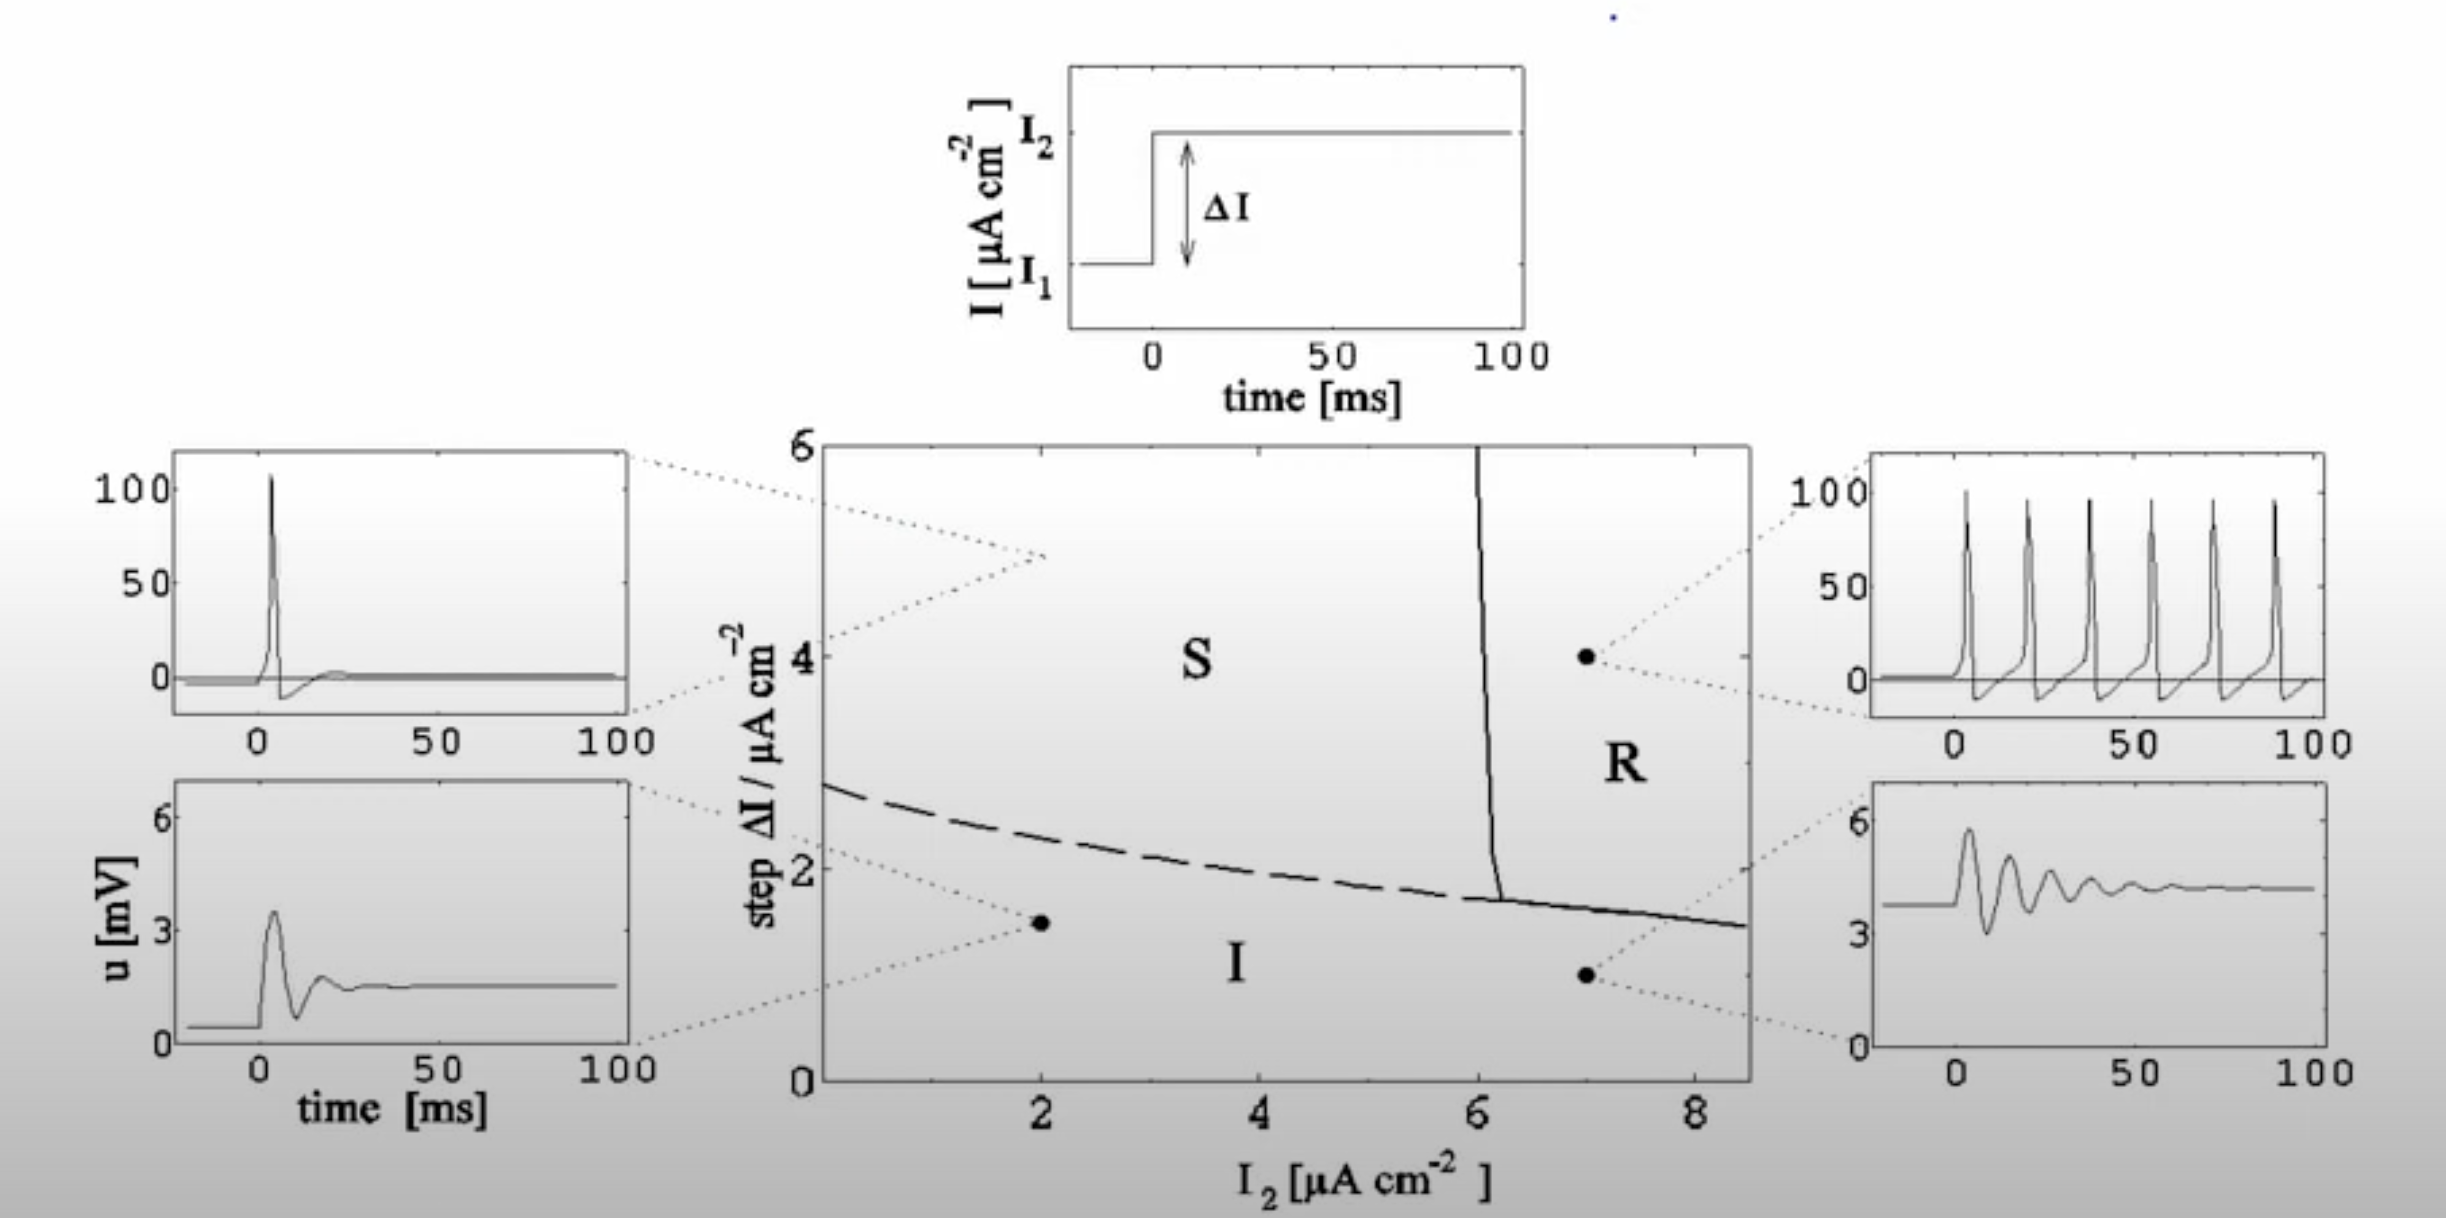
\includegraphics[scale=0.3]{2.4.png}
    \end{center}
    \begin{enumerate}
        \item What do the horizontal axis ($I_2$) and the vertical axis (step $\Delta I$) represent in this plot?
        \vspace{3 cm}
        \item Based on this parameter space, what shape does the current step function need to have to cause a neuron to fire repetitively?
    \end{enumerate}
\end{enumerate}
\pagebreak

\section{CNS2.5 - Detailed Biophysical Models}
\begin{enumerate}
    \item The lecture introduces two sources of adaptation that can lead to an elongation of inter-spike intervals. Provide a concise summary of each adaptation source:
    \begin{enumerate}
        \item $I_M$ Slow potassium current:
        \vspace{3 cm}
        \item $I_{NaP}$ Persistent sodium current: 
    \end{enumerate}
\end{enumerate}

\pagebreak

\section{V\&B Chapter 2 - Eyes}
\begin{enumerate}
    \item The evolution of the eye into a cup shape has significant implications for visual perception. Why is this morphological development crucial?
    \begin{enumerate}
        \item[a.] The cup shape allows the eye to store more light, enabling brighter vision.
        \item[b.] The cup shape provides the eye a larger surface area, allowing for a wider field of vision.
        \item[c.] The cup shape allows the eye to better determine the direction of incoming light, enhancing the animal's ability to sense the direction of light sources.
        \item[d.] The cup shape enhances the eye's ability to change focus between near and distant objects.
    \end{enumerate}

    \item Which of the following statements about a pinhole camera is true?
    \begin{enumerate}
        \item[a.] The smaller the pinhole, the better the image clarity in all circumstances.
        \item[b.] Shrinking the pinhole too much can lead to the appearance of diffraction patterns that can degrade the image quality.
        \item[c.] The quality of the image in a pinhole camera is primarily determined by the focal length.
        \item[d.] The larger the pinhole, the brighter the image without any degradation in its sharpness.
    \end{enumerate}

    \item The orientation of human photoreceptors, facing towards the back of the retina, with other neurons like ganglion cells situated closer to incoming light, is a unique arrangement. The author does not provide a reason for this orientation. Conduct some research or consult ChatGPT. What are some possible explanations for this photoreceptor arrangement in humans? Provide a brief summary of your findings.
    \vspace{3 cm}

    \item We humans often perceive green as being brighter than blue even when the two colors are equally bright. What might be the reason for this?
    \begin{enumerate}
        \item[a.] The human eye has more green cones than blue cones.
        \item[b.] The wavelength of green light is longer than that of blue light, making it appear brighter.
        \item[c.] Our perception of brightness is influenced by the distribution of cones in our retina, which is optimized for daylight conditions where green is the most prevalent color.
        \item[d.] Blue light is absorbed more by the atmosphere, making it appear less bright to us.
    \end{enumerate}

    \item In Figure 2.12, the author uses degrees as the unit of retinal eccentricity. This measure is essentially referring to a concept known as visual angle. What does the visual angle represent in this context?
    \begin{enumerate}
        \item[a.] It represents the angle formed by the lens of the eye as it adjusts to focus light on the retina.
        \item[b.] It refers to the angle subtended at the eye by an object in the visual field, indicating the size of the object's image on the retina.
        \item[c.] It represents the angle of deviation of the eyes when looking at objects in the peripheral field of view.
        \item[d.] It corresponds to the angle of incidence of light as it strikes the cornea.
    \end{enumerate}
\end{enumerate}

\end{document}